
\begin{figure}
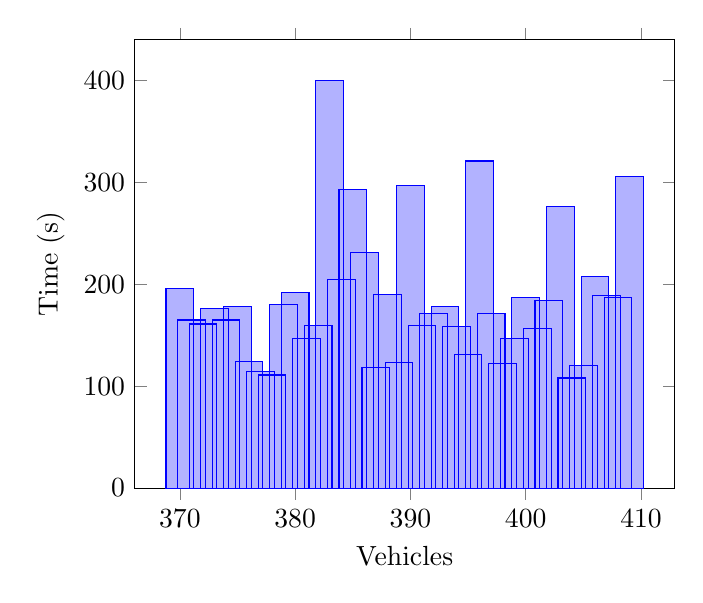
\begin{tikzpicture}
\begin{axis}[
legend style={anchor=west},
xlabel=Vehicles,
ylabel=Time (s),
ymin=0,
ybar,
]
\addplot coordinates {
(409, 306)
(407, 189)
(406, 208)
(405, 120)
(403, 276)
(402, 184)
(401, 157)
(400, 187)
(379, 180)
(378, 111)
(370, 196)
(377, 114)
(376, 124)
(393, 178)
(392, 171)
(397, 171)
(396, 321)
(395, 131)
(394, 159)
(398, 122)
(391, 160)
(380, 192)
(381, 147)
(382, 160)
(383, 400)
(384, 205)
(385, 293)
(386, 231)
(387, 118)
(388, 190)
(389, 123)
(404, 108)
(408, 187)
(371, 165)
(373, 176)
(375, 178)
(374, 165)
(390, 297)
(372, 161)
(399, 147)
};

\end{axis}
\end{tikzpicture}
\label{tik:time:100:96}
\caption{100 percent diving with GSC on route $96$}
\end{figure}
